%------------------------------------------------------------------------------
% CV in Latex
% Author : Charles Rambo
% Based off of: https://github.com/sb2nov/resume and Jake's Resume on Overleaf
% Most recently updated version may be found at https://github.com/fizixmastr 
% License : MIT
%------------------------------------------------------------------------------

\documentclass[A4,11pt]{article}
%\documentclass[letterpaper,11pt]{article} %For use in US
\usepackage{latexsym}
\usepackage[empty]{fullpage}
\usepackage{titlesec}
\usepackage{marvosym}
\usepackage[usenames,dvipsnames]{color}
\usepackage{verbatim}
\usepackage{enumitem}
\usepackage[hidelinks]{hyperref}
\usepackage[english]{babel}
\usepackage{tabularx}
\usepackage{tikz}
\input{glyphtounicode}

\begin{comment}
I am by no means a professional when it comes to the CV's/resumes, I have
received various trainings on how to write a CV and resume from my high 
school, as well as the Austin College and University of Eastern Finland's
career counseling departments. As I intend to share my CV as a template, I 
feel that it is my responsibility to provide explanations of my work.
\end{comment}


%-----FONT OPTIONS-------------------------------------------------------------
\begin{comment}
The font of the document will impact not just how readable it is, but how it is
perceived. In the "The Craft of Scientific Writing" by Michael Alley, shares a
common fonts for publication as well as their use. I have chosen to use
Palatino for its legibility, some others are given below. There is far too much
about typography to discus here. Note: serif fonts have short projecting
strokes, sans-serif fonts are sans (without) these strokes.
\end{comment}


% serif
 \usepackage{palatino}
% \usepackage{times} %This is the default as well
% \usepackage{charter}

% sans-serif
% \usepackage{helvet}
% \usepackage[sfdefault]{noto-sans}
% \usepackage[default]{sourcesanspro}

%-----PAGE SETUP---------------------------------------------------------------

% Adjust margins
\addtolength{\oddsidemargin}{-1cm}
\addtolength{\evensidemargin}{-1cm}
\addtolength{\textwidth}{2cm}
\addtolength{\topmargin}{-1cm}
\addtolength{\textheight}{2cm}

% Margins for US Letter size
%\addtolength{\oddsidemargin}{-0.5in}
%\addtolength{\evensidemargin}{-0.5in}
%\addtolength{\textwidth}{1in}
%\addtolength{\topmargin}{-.5in}
%\addtolength{\textheight}{1.0in}

\urlstyle{same}

\raggedbottom
\raggedright
\setlength{\tabcolsep}{0cm}

% Sections formatting
\titleformat{\section}{
  \vspace{-4pt}\scshape\raggedright\large
}{}{0em}{}[\color{black}\titlerule \vspace{-5pt}]

% Ensure that .pdf is machine readable/ATS parsable
\pdfgentounicode=1

%-----CUSTOM COMMANDS FOR FORMATTING SECTIONS----------------------------------
\newcommand{\CVItem}[1]{
  \item\small{
    {#1 \vspace{-2pt}}
  }
}

\newcommand{\CVSubheading}[4]{
  \vspace{-2pt}\item
    \begin{tabular*}{0.97\textwidth}[t]{l@{\extracolsep{\fill}}r}
      \textbf{#1} & #2 \\
      \small#3 & \small #4 \\
    \end{tabular*}\vspace{-7pt}
}
\newcommand{\medi}[3]{
  \vspace{-2pt}\item
    \begin{tabular*}{0.97\textwidth}[t]{l@{\extracolsep{\fill}}r}
      \textbf{#2} & #1 \\
      \small#3 \\
    \end{tabular*}\vspace{-7pt}
}
\newcommand{\CVSubheadingshort}[2]{
  \vspace{-2pt}\item
    \begin{tabular*}{0.97\textwidth}[t]{l@{\extracolsep{\fill}}r}
      \textbf{#1} & #2 \\
    \end{tabular*}\vspace{-7pt}
}
\newcommand{\CVSubSubheading}[2]{
    \item
    \begin{tabular*}{0.97\textwidth}{l@{\extracolsep{\fill}}r}
      \text{\small#1} & \text{\small #2} \\
    \end{tabular*}\vspace{-7pt}
}

\newcommand{\CVSubItem}[1]{\CVItem{#1}\vspace{-4pt}}

\renewcommand\labelitemii{$\vcenter{\hbox{\tiny$\bullet$}}$}

\newcommand{\CVSubHeadingListStart}{\begin{itemize}[leftmargin=0.5cm, label={}]}
% \newcommand{\resumeSubHeadingListStart}{\begin{itemize}[leftmargin=0.15in, label={}]} % Uncomment for US
\newcommand{\CVSubHeadingListEnd}{\end{itemize}}
\newcommand{\CVItemListStart}{\begin{itemize}}
\newcommand{\CVItemListEnd}{\end{itemize}\vspace{-5pt}}

%------------------------------------------------------------------------------
% CV STARTS HERE  %
%------------------------------------------------------------------------------
\begin{document}

%-----HEADING------------------------------------------------------------------
\begin{comment}
In Europe it is common to include a picture of ones self in the CV. Select
which heading appropriate for the document you are creating.
\end{comment}

\begin{minipage}[c]{0.05\textwidth}
\-\
\end{minipage}
\begin{minipage}[c]{0.2\textwidth}
\begin{tikzpicture}
    \clip (0,0) circle (1.75cm);
    \node at (0,-.3) {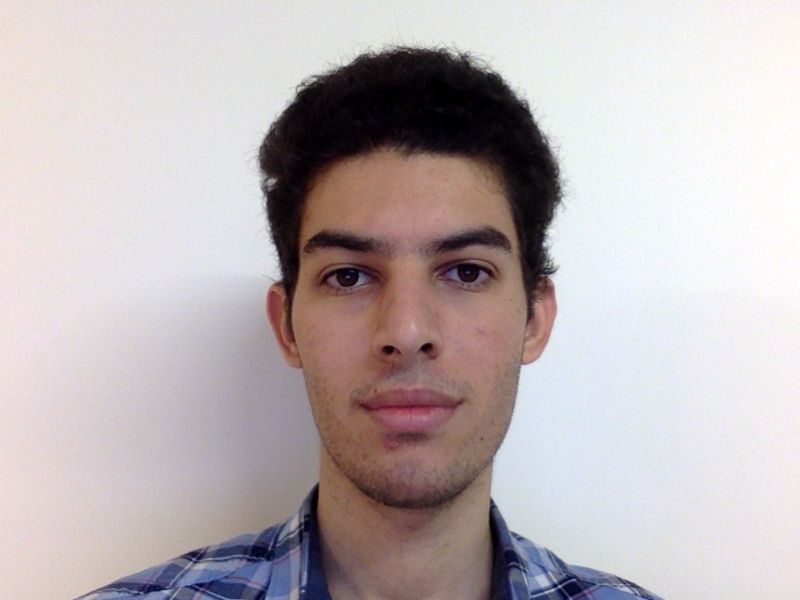
\includegraphics[width = 5cm]{moi}}; 
    % if necessary the picture may be moved by changing the at (coordinates)
    % width defines the 'zoom' of the picture
\end{tikzpicture}
\hfill\vline\hfill
\end{minipage}
\begin{minipage}[c]{0.6\textwidth}
    \textbf{\Huge \scshape{Omar Mohsen}} \\ \vspace{1pt} 
    % \scshape sets small capital letters, remove if desired
    \small{+33 7 81 32 99 93} \\\small{01 Mars 1996}\\
    \small{French and Egyptian}\\
    \href{https://www.imo.universite-paris-saclay.fr/fr/}{Maître de conférence at universite of Paris-Saclay}\\
   \href{mailto:omar.mohsen@universite-paris-saclay.fr}{omar.mohsen (AT) universite-paris-saclay.fr}\\ \href{https://sites.google.com/view/omar-mohsen-webpage/home}{https://sites.google.com/view/omar-mohsen-webpage/home} \\
\end{minipage}

% Without picture
%\begin{center}
%    \textbf{\Huge \scshape Charles Rambo} \\ \vspace{1pt} %\scshape sets small capital letters, remove if desired
%    \small +1 123-456-7890 $|$ 
%    \href{mailto:you@provider.com}{\underline{you@provider.com}} $|$\\
%    % Be sure to use a professional *personal* email address
%    \href{https://linkedin.com/in/your-name-here}{\underline{linkedin.com/in/charles-rambo}} $|$
%    % you should adjust you linked in profile name to be professional and recognizable
%    \href{https://github.com/fizixmastr}{\underline{github.com/fizixmastr}}
%\end{center}



%-----EDUCATION----------------------------------------------------------------
\section{Scientific Career}
  \CVSubHeadingListStart
\CVSubheading
      {{Maître de conférence (research/teaching position)}}{September. 2019 -- Current}
      {University of Paris-Saclay}{France}   
    \CVSubheading
      {{Postdoc}}{September. 2019 -- August 2021}
      {University of Muenster}{Germany}
        \CVSubheading
      {{ATER (Teaching Position)}}{October 2018 -- August 2019}
      {Université Paris Diderot}{France}
  \CVSubHeadingListEnd
\section{Education}
  \CVSubHeadingListStart
    \CVSubheading
      {{PhD $|$ \emph{\small{Thesis defended in October 2018 under the direction of G. Skandalis}}}}{October 2015 -- October 2018}
      {Université Paris Diderot}{France}
    \CVSubheading
      {{ENS Diploma}}{2012 -- 2015}
      {École normale supérieure de Paris}{France}
    \CVSubheading
      {Master}{2013 -- 2015}
      {University of Paris-Saclay}{France}
  \CVSubHeadingListEnd

\section{Published articles}
  \CVSubHeadingListStart
    \CVSubheading
      {Witten deformation using Lie groupoids}{2021}
      {Advances in Mathematics}{}  
    \CVSubheading
      {The convolution algebra of Schwarz kernels on a singular foliation}{2020}{Journal of Operator theory}{with Androulidakis and Yuncken}
    \CVSubheading
      {On the deformation groupoid of the inhomogeneous pseudo-differential calculus}{2020}
      {Bulletin of the London Mathematical society}{}
    \CVSubheading
      {Chern Simons invariants in $K\!K$ theory}{2018}
      {Journal of functional analysis}{}
  \CVSubheading
      {Index theorem for inhomogeneous hypoelliptic differential operators}{2020}
      {Muenster Journal of Mathematics}{}

  \CVSubHeadingListEnd

%-----PROJECTS AND RESEARCH----------------------------------------------------
\begin{comment}
Ideally the title of the work should speak for what it is. However if you feel
like you should explain more about why the project is applicable to this job,
use item list as is shown in the work experience section.
\end{comment}

\section{Prepublication Articles}
  \CVSubHeadingListStart
%    \CVSubheading
%      {Title of Work}{When it was done}
%      {Institution you worked with}{unused}
 \CVSubheading
   {Tangent groupoid and tangent cones in sub-Riemannian geometry}{2022}
    {}{}  
 \CVSubheading
   {Higher order derivations on C*-algebras and applications to smooth functional calculus}{2022}
    {}{}  
  \CVSubheading
   {On the index of maximally hypoelliptic differential operators}{2022}
    {}{}
 \CVSubheading
      {A pseudodifferential calculus for maximally hypoelliptic operators and the Helffer-Nourrigat conjecture}{}
      {with Androulidakis and Yuncken 2022}{}   
 \CVSubheading
   {Blow-up groupoid of singular foliations}{2022}
    {}{}    
    
  \CVSubHeadingListEnd
%------------------------------------------------------------------------------
\end{document}